\begin{center}
	\begin{picture}(\spaltenbreite,21)
	\put(-4,13){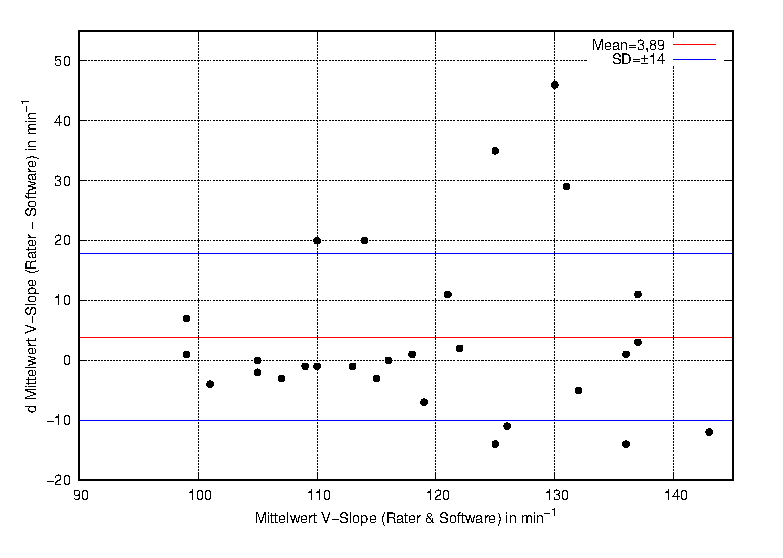
\includegraphics[width=110mm]{Bilder/vslope.eps}}
	\put(-0.8,12){\parbox{720pt}{{\bf \small a)} \small für V-Slope}}
	\put(8,13){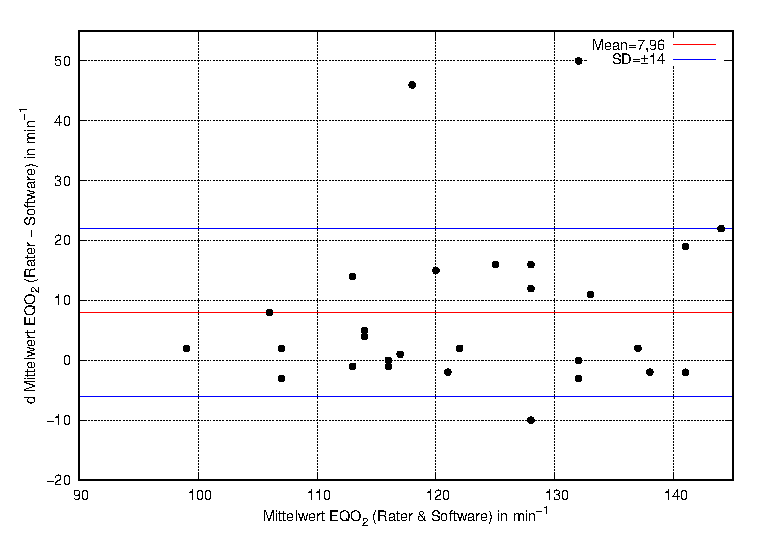
\includegraphics[width=110mm]{Bilder/eqo2.eps}}
	\put(11.5,12){\parbox{720pt}{{\bf \small b)} \small für EQO\textsubscript{2}}}
	\put(-4,3){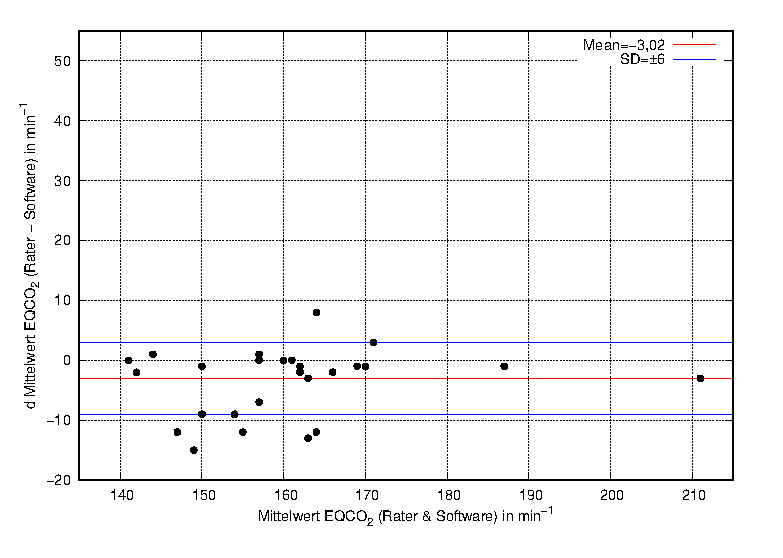
\includegraphics[width=110mm]{Bilder/eqco2.eps}}
	\put(-0.7,2){\parbox{720pt}{{\bf \small c)} \small für EQCO\textsubscript{2}}}
	\put(8,3){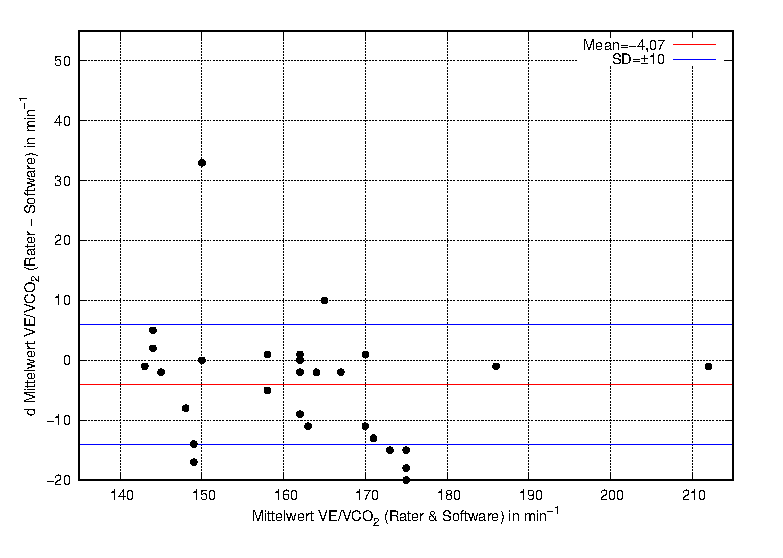
\includegraphics[width=110mm]{Bilder/vevco2.eps}}
	\put(11,2){\parbox{720pt}{{\bf \small d)} \small für \.{V}E/\.{V}CO\textsubscript{2}}}
	\put(-2.6,0.6){\parbox{720pt}{{\bf \small Abb. 7:} \small Streuung der Ergebnisse um die mittlere Abweichung}}
	\end{picture}
\end{center}
\vspace{1em}
Die Abb. 7 zeigt zu diesen Ergebnissen die methodenspezifische Streuung der Schwellenbestimmungen um die mittlere Abweichung zzgl. der entsprechenden Standardabweichung (SD).
\vspace{1.5em}

